\documentclass[12pt, a4paper, openany]{report}

\def\VersionRapport{1.0}

\usepackage[utf8]{inputenc} % un package
\usepackage[T1]{fontenc}      % un second package
\usepackage[francais]{babel}  % un troisième package
\usepackage{layout}
\usepackage[top=2.7cm, bottom=2.5cm, left=3.5cm, right=3cm]{geometry}
\usepackage{setspace}

\frenchbsetup{StandardLists=true} % à inclure si on utilise \usepackage[french]{babel}
%\usepackage{enumitem}
\usepackage[shortlabels]{enumitem}
\usepackage{amssymb}

\usepackage{color}
\usepackage{listings}
\definecolor{dkgreen}{rgb}{0,0.6,0}
\definecolor{gray}{rgb}{0.5,0.5,0.5}
\definecolor{mauve}{rgb}{0.58,0,0.82}

\lstset{frame=tb,
  language=Java,
  aboveskip=3mm,
  belowskip=3mm,
  showstringspaces=false,
  columns=flexible,
  basicstyle={\small\ttfamily},
  numbers=none,
  numberstyle=\tiny\color{gray},
  keywordstyle=\color{blue},
  commentstyle=\color{dkgreen},
  stringstyle=\color{mauve},
  breaklines=true,
  breakatwhitespace=true,
  tabsize=3
}

\usepackage{multirow} % pour les tableaux
\usepackage[table]{xcolor} % pour les tableaux

\usepackage{verbatim}
\usepackage{moreverb}
\usepackage{url}
\usepackage{pst-all}
\usepackage{eso-pic,graphicx}
\usepackage{caption} 
\usepackage[colorlinks=true,urlcolor=blue,linkcolor=red]{hyperref}
\usepackage{array}
\usepackage[toc,page]{appendix}
\usepackage[off]{auto-pst-pdf}
\usepackage{hyperref} % pour le sommaire table des matières
\AddThinSpaceBeforeFootnotes % à insérer si on utilise \usepackage[french]{babel}
\FrenchFootnotes % à insérer si on utilise \usepackage[french]{babel}
\usepackage{fancyhdr}
\pagestyle{headings}
\usepackage{pifont}  %pour les puces
\usepackage{amsmath} %pour les puces

\usepackage{verbatim} % pour le code en annexe 

%%%%%%%colones 
\newcolumntype{R}[1]{>{\raggedleft\arraybackslash }b{#1}}
\newcolumntype{L}[1]{>{\raggedright\arraybackslash }b{#1}}
\newcolumntype{C}[1]{>{\centering\arraybackslash }b{#1}}
%%%%%%% 

\renewcommand{\appendixpagename}{Annexes}
\renewcommand{\appendixtocname}{Annexes}

\title{Theme: Compte Rendu Système Linéaire à Temps Continu 1}
\author{REBOUT \bsc{Mehenna}}
\author{BOUYOUCEF \bsc{Farid}}
\date{2018-2019}



%new
\newcommand{\HRule}{\rule{\linewidth}{0.5mm}}


\begin{document}

%\selectlanguage{francais}
\pagenumbering{arabic} 

\makeatletter
  \begin{titlepage}
  

  \begin{sffamily}
   \begin{center}

    % Upper part of the page. The '~' is needed because \\
    % only works if a paragraph has started.
    
\includegraphics[scale=0.5]{Logo_UT3.jpg}~\\[1.5cm]

    \textsc{\LARGE Master 1 EEA ISTR/RODECO  }\\[2cm]

    \textsc{\Large Compte Rendu  Système Linéaire à Temps Continu 1}\\[1.5cm]

    % Title
    \HRule \\[0.4cm] % saut de ligne
    { \huge \bfseries TP 1 Pendule\\[0.4cm] }

    \HRule \\[1cm]   % sous de ligne 
    
\includegraphics[scale=0.1]{logomaster.jpg}
    \\[1cm]

    % Author and supervisor
    \begin{minipage}{0.4\textwidth}
      \begin{flushleft} \large
         \textsc{\emph {Réalisés par:} \\REBOUT Mehenna}\\
         \textsc{BOUYOUCEF Farid}   
          \newline
          Promotion 2018-2019 \\
      \end{flushleft}
    \end{minipage}
    \begin{minipage}{0.4\textwidth}
      \begin{flushright} \large
        \emph{Tuteur :}  \textsc{M DUROLA}\\
        \emph{Responsable de la Formation:} \textsc{M GOUAISBAUT}
      \end{flushright}
    \end{minipage}

    \vfill

    % Bottom of the page
    {\large Octobre 2018}

  \end{center}
  \end{sffamily}      
          
  \end{titlepage}
  
\makeatother




   
%*********************** somaire **************
\renewcommand{\contentsname}{Sommaire}
\tableofcontents
%*********************** listes des figures **************
\listoffigures
%*********************** listes des tableaux **************
\listoftables



%*********************** INTRODUCTION **************
\chapter*{Introduction}Dans ce TP on va réaliser un asservissement de position ,on va utiliser pour cette manipulation la platine voir   la Figure 1.1.
\addcontentsline{toc}{chapter}{Introduction}

\begin{center}
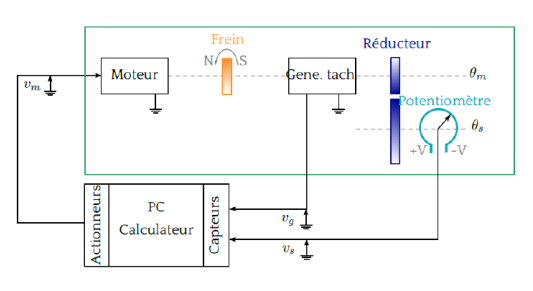
\includegraphics[scale=0.5]{fiiig1.png}
\captionof{figure}{\textit{Asservissement de position par calculateur}}
\label{fig1} 
\end{center}

Les valeurs numériques des coefficients connus sont:\\

 $K_e=10(V.tr^-1)$	 \hfill		$K_s=10(V.tr^-1)$	\hfill		$Kg=0.105(V.s.tr^-1)$ 
 
 
    \chapter{ PRÉLIMINAIRE DU PROCÉDÉ}
     \section{Représentation et analyse de ensemble (moteur, réducteur, potentiomètre, génératrice        tachymétrique) pour le système $ {S_V}_m \rightarrow V_S$ }
 

\begin{center}
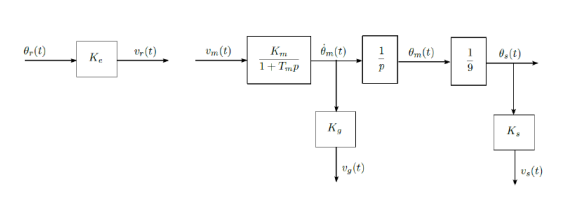
\includegraphics[scale=0.5]{fiiig2.png}
\captionof{figure}{\textit{ Eléments de la platine "asservissement de positon"}}
\label{fig1} 
\end{center}

On considère le système en boucle ouverte l’entrée du système on boucle ouvert est $V_m(t)$ et la sortie mesurée $V_s(t)$, que l’on note  par $ {S_V}_m \rightarrow V_S$.


\subsection{la représentation d’état de ce système, lorsque son vecteur d’état est défni par:}


\begin{equation}
x(t)={(x_1(t),x_2(t))}^T={(V_s(t),V_g(t))}^T
\end{equation}
$x_1=V_s$ et $x_2=V_g$
\\\\


$x_1=\frac{K_s}{9p}\frac{x_2}{K_g}$\\
$\frac{x_2}{K_g}=\frac{K_m}{1+T_m}$
\\
\\

\begin{equation*}
\left\{\begin{matrix}
\dot{x}(t)=Ax(t)+Bu(t)\\ 
y(t)=Cx(t)+Du(t)\\
\end{matrix}\right.
\end{equation*}   

%%%%%%%%%%%comment je vais faire les []%%%%%%%%%
$\dot{X}$=$$\begin{matrix}0&\frac{K_s}{9K_g}\\0&-\frac{1}{T_m}\end{matrix}x$$
\quad+\quad $$\begin{matrix}0
\frac{K_mK_g}{T_m}
\end{matrix}V_m
$$
\\\\

avec U=Vm , Y=Vs, X est le vecteur d'état\\
D'où: Il n y a  pas de transfert direct en boucle ouvert car D=0\\
alors: $$y=[1\quad0].X$$ 



\subsection{Détermination des pont d’équilibre lorsque $v_m$(t) est constante, et L’étude de stabilité }

\begin{center}
$\dot{X}_eq=0$
\end{center}

\begin{center}
$x_2=0 $\\
$x_2=K_g.K_m.V_m$ \\
\end{center}

\begin{center}
si $V_m$ $\ne $0 donc il n y a pas de point d'équilibre \\
si $V_m$=0 alors\\
 $\dot{X}_eq=$ \end{center}$$\begin{pmatrix} 0\\\alpha \end{pmatrix}$$
 
 \begin{center}
avec $\alpha$ $\in$ R
\end{center}


%%******************* Coclusion
\chapter*{Conclusion}
\addcontentsline{toc}{chapter}{Conclusion}

Ce TP nous a permet d'utiliser les différentes commandes de robustesse et a appris de définir un correcteur par étapes, cela en vérifiant chaque contrainte pour déterminer un meilleur correcteur.\\










\begin{appendices}
\chapter*{Annexe 1}
	
				
\end{appendices}





%Bibliographie 
%\bibliographystyle{alpha}
%\bibliography{biblio}




\end{document}







